\documentclass[journal,12pt,twocolumn]{IEEEtran}
\usepackage{hyperref}
\usepackage{graphicx}
\title{Assignment 1}
\author{JARPULA BHANU PRASAD - AI21BTECH11015	}
\date{April 2021}
\begin{document}
\maketitle
\Large \underline{Download codes from}:\\
\large Python code for graph - \href{https://github.com/jarpula-Bhanu/Assinment-1/blob/main/quardratic.py}{python}.\\And c-code for roots -  \href{https://github.com/jarpula-Bhanu/Assinment-1/blob/main/roots.c}{c-code}.\\And latex code from - \href{https://github.com/jarpula-Bhanu/Assinment-1/blob/main/Assignment_1.tex}{Latex}.

\section{\Large \underline{Problem-ICSE-2019-10  Q)4-b}}
\large \noindent Q)Solve for $x$ the quadratic equation $$x^2-4x-8=0.$$ Give your answer correct to three significant figures.
\section{\large \underline{solution}}
Given quadratic equation,
\large $$x^2-4x-8=0.$$
Solution for the quadratic equation is the form  \large $$ax^2+bx+c=0$$ is given by 
\begin{center}
\framebox[1.1\width]{\LARGE $\frac{-b\pm\sqrt{b^2-4ac}}{2a}$}
\end{center}

let $\alpha$ and $\beta$ be the roots of the equation,\\Such that,
\begin{center}
\framebox[1.1\width]{$\alpha$ =\Large $\frac{-b+\sqrt{b^2-4ac}}{2a}$ and  $\beta$ =\Large $\frac{-b-\sqrt{b^2-4ac}}{2a}$}
\end{center}

Now, from given equation \\$a$=1,$b$=-4 and $c$=-8.
\begin{center}
$\alpha$ =\Large $\frac{-(-4)+\sqrt{(-4)^2-4(1)(-8)}}{2(1)}$
\end{center}
and
\begin{center}
$\beta$ =\Large $\frac{-(-4)-\sqrt{(-4)^2-4(1)(-8)}}{2(1)}$
\end{center}

On simplifying we get,
\begin{center}
$\alpha$=2+2$\sqrt{3}$  and $\beta$=2-2$\sqrt{3}$ 
\end{center}
i.e., The roots of the equation are,
\begin{center}
$\alpha$=5.464 and $\beta$=-1.464
\end{center}
On rounding off to three significant figures.
\\The roots of the equation are,
\begin{center}
\framebox[1.1\width]{$\alpha$=5.46 and $\beta$=-1.46.}
\end{center}
\begin{figure}[h] 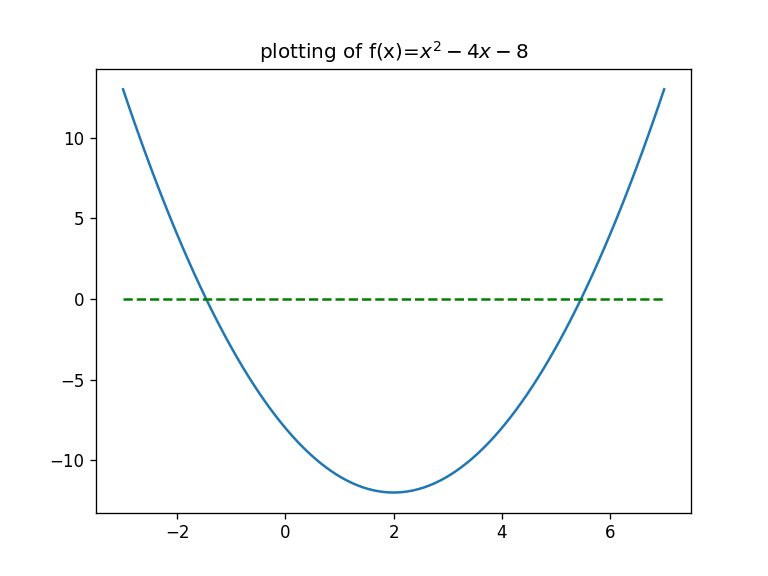
\includegraphics[scale=0.65]{Figure_0}\large \caption{Roots of the equation}
\end{figure}

\noindent The above graph gives the roots of the equation

 


\end{document}
